\documentclass[a4paper, 9pt]{article}
\usepackage[latin1]{inputenc}
\usepackage[T1]{fontenc}
\usepackage[francais]{babel}
\usepackage{entete}
\usepackage{noitemsep}
\usepackage{euscript} 
\usepackage{amsmath,amssymb,amsfonts,amsthm}
\usepackage{graphicx,graphics,epsfig,subfigure,color}
\usepackage{url}
%\usepackage{algorithm2e}
\usepackage{multicol}
\usepackage{a4wide}
\usepackage{latexsym}
\usepackage{verbatim}
\setlength{\textheight}{24cm}
\setlength{\topmargin}{-0.5cm}
\setlength{\textwidth}{160mm}
\setlength{\oddsidemargin}{1mm}

%\renewcommand{\baselinestretch}{0.85}

%\input{macroAlgo}
%\dontprintsemicolon

\setlength{\parindent}{0pt}  %%suppression indentation


\begin{document}
\selectlanguage{francais}
\author{D. Fourer, L. Lagon}
\newcommand{\universityname}{IUT d'\'Evry Val d'Essonne}
\newcommand{\deptname}{D\'epartement TC (S1)}
\newcommand{\years}{2023-2024}

%------------------- TITRE -----------------------------------------
\date{Septembre 2023} 
\TDHead{\universityname}{\deptname}{R1.13, Ressources et Culture Num\'eriques 1, \years}{\large TD3 : Pr\'esentation professionnelle}
%\TDHead{DUT TC}{}{\large TIC3: Fonctions avanc\'ees d'un tableur}
%-------------------------------------------------------------------
\underline{Objectifs:} Cr\'eer une pr\'esentation professionnelle de votre entreprise (FA) ou de l'entreprise de votre choix (FI). 
\flushleft
\vspace{-0.2cm}

\exost Lancez le logiciel de votre choix (Libreoffice Impress ou PowerPoint) et cr\'eez une pr\'esentation de votre entreprise contenant au minimum 15 diapositives .
Votre pr\'esentation respectera les consignes suivantes:
\begin{itemize}
 \item Votre pr\'esentation respectera le plan suivant :  
 \begin{enumerate}
  \item Activit\'e
  \item Organigramme
  \item analyse SWOT\footnote{forces/faiblesses/opportunit\'es/menaces}
  \item vos missions
  \item r\'ealisations
  \item perspectives
  \end{enumerate}
 \item Votre pr\'esentation comportera une diapositive de titre comportant votre nom et celle de votre entreprise, ainsi qu'une table des mati\`eres
 \item Vous int\'egrerez plusieurs images dans votre pr\'esentation, dont le logo de l'IUT et celui de votre entreprise
 \item Vous utiliserez au minimum 2 transitions diff\'erentes permettant de rendre votre diaporama plus attrayant
 \item Votre diaporama comportera au moins une vid\'eo dans l'une des diapositives
\end{itemize}

\exost Cr\'eez un masque des diapositives original permettant d'obtenir un style personnalis\'e pour votre pr\'esentation.\\
\centering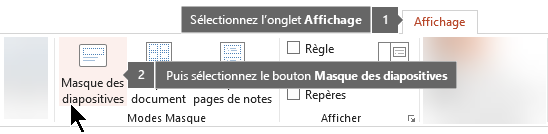
\includegraphics[width=0.8\textwidth]{./masque.png}
\flushleft

\exost Ins\'erez la date, l'heure et le num\'ero de chaque diapositive en bas \`a droite de votre pr\'esentation.

\exost Enregistrez votre pr\'esentation dans chacun des 3 formats suivants: PPTX, PPSX et PDF.
R\'eouvrez chaque fichier obtenu puis expliquez les diff\'erences et l'int\'er\^et de chacun de ces trois formats.

\exost Mettez votre pr\'esentation en ligne sur le cloud de votre choix (eg. google drive) pour permettre \`a plusieurs utilisateurs de travailler 
simultan\'ement dessus tout en gardant un historique des modifications.

\end{document}

% End Of File

